\begin{Pro}
Del ejercicio anterior, utiliza las regex de las expresiones booleanas para definir el AF, conviértelo en AFD y redúcelo. Pruébalo con las siguientes expresiones para obtener los tokens:

\begin{enumerate}
    \item[(a)] $p \land q$
    \item[(b)] $\textbf{True} \land \lnot(p \lor q)$
    \item[(c)] $\lnot(x \land y) \lor (p \land q)$
\end{enumerate}

\end{Pro}


Para convertirlo en AF usando Thompson creamos un estado inicial y un estado final, y vamos añadiendo los estados y transiciones según las regex que definimos en el ejercicio anterior. Con lo que obtenemos:

\begin{figure}[H]
    \centering
    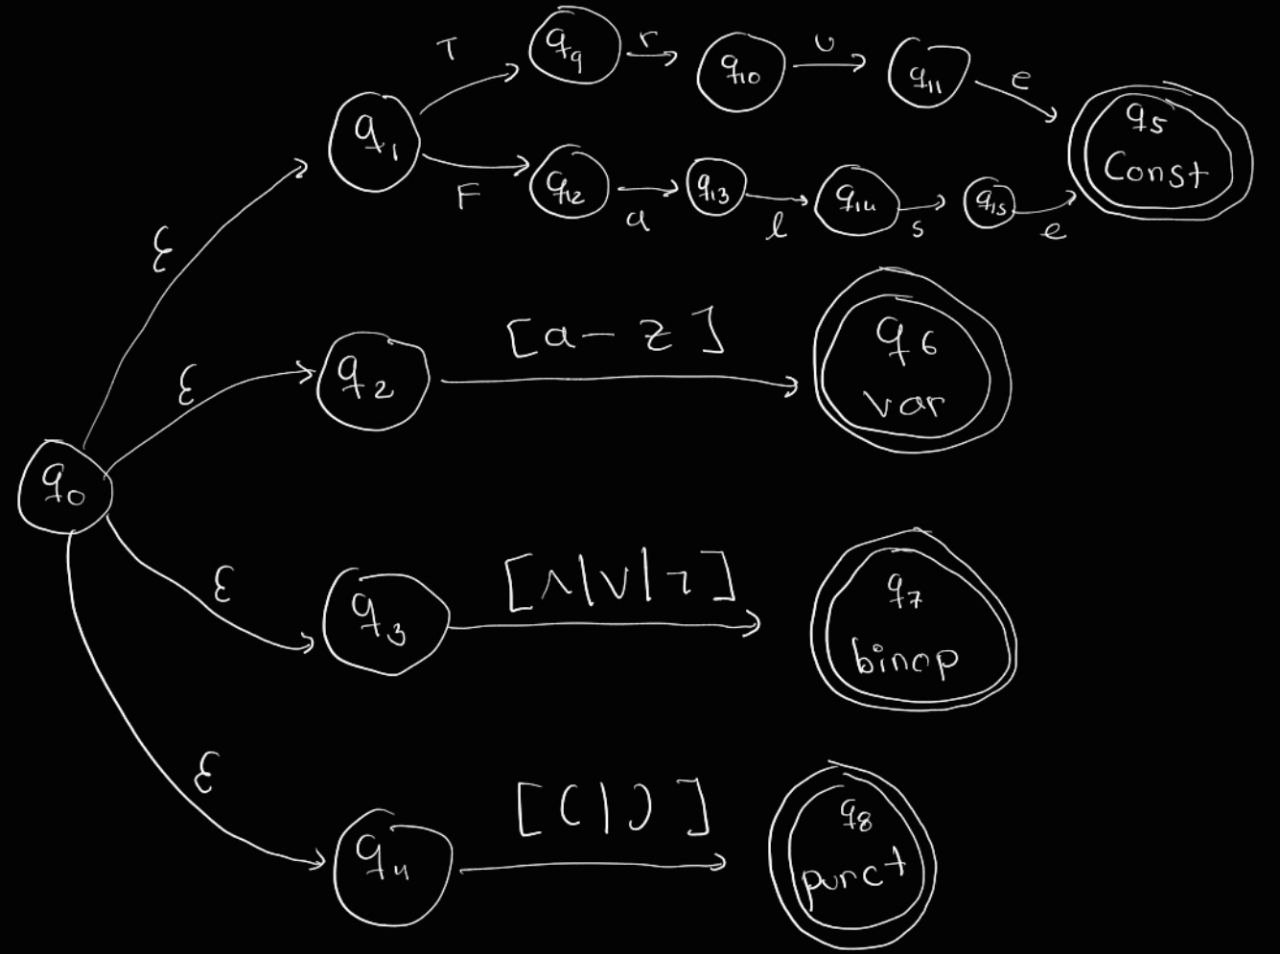
\includegraphics[width=0.8\textwidth]{images/ejercicio10-1.jpg}
    \caption{AF para lexer expresiones booleanas}
    \label{fig:my_label}
\end{figure}


Primero vamos a obtener la epsilon-cerradura de cada uno de los estados:

\begin{itemize}
    \item $\epsilon-closure(\{q_0\}) = \{q_0, q_1, q_2, q_3, q_4\}$
    \item $\epsilon-closure(\{q_1\}) = \{q_1\}$
    \item $\epsilon-closure(\{q_2\}) = \{q_2\}$
    \item $\epsilon-closure(\{q_3\}) = \{q_3\}$
    \item $\epsilon-closure(\{q_4\}) = \{q_4\}$
    \item $\epsilon-closure(\{q_5\}) = \{q_5\}$
    \item $\epsilon-closure(\{q_6\}) = \{q_6\}$
    \item $\epsilon-closure(\{q_7\}) = \{q_7\}$
    \item $\epsilon-closure(\{q_8\}) = \{q_8\}$
    \item $\epsilon-closure(\{q_9\}) = \{q_9\}$
    \item $\epsilon-closure(\{q_{10}\}) = \{q_{10}\}$
    \item $\epsilon-closure(\{q_{11}\}) = \{q_{11}\}$
    \item $\epsilon-closure(\{q_{12}\}) = \{q_{12}\}$
    \item $\epsilon-closure(\{q_{13}\}) = \{q_{13}\}$
    \item $\epsilon-closure(\{q_{14}\}) = \{q_{14}\}$
    \item $\epsilon-closure(\{q_{15}\}) = \{q_{15}\}$
\end{itemize}

Ahora vamos a obtener las transiciones de cada uno de los estados:

\begin{table}[h!]
\centering
\begin{tabular}{|c|c|c|c|c|c|c|c|c|c|c|c|c|}
\hline
Estado &T & r & u & e & F & a & l &s &[a-z]-[r,u,e,a,l,s] &$\land/\lor/\lnot$ & (, )\\ \hline
\hline
$\{q_0, q_1, q_2, q_3, q_4\}$ & $\{q_9\}$ & $\{q_6\}$ & $\{q_6\}$ & $\{q_{6}\}$ & $\{q_{12}\}$ & $\{q_6\}$ & $\{q_6\}$ & $\{q_6\}$ & $\{q_6\}$ & $\{q_7\}$& $\{q_8\}$\\ \hline
\end{tabular}
\end{table}

En este punto tenemos como nuevos estados $\{q_6\}, \{q_7\}, \{q_8\}, \{q_9\}, \{q_{12}\}$. Vamos a agregarlos a la tabla de transiciones:

\begin{table}[h!]
\centering
\begin{tabular}{|c|c|c|c|c|c|c|c|c|c|c|c|c|}
\hline
Estado &T & r & u & e & F & a & l &s &[a-z]-[r,u,e,a,l,s] &$\land/\lor/\lnot$ & (, )\\ \hline
\hline
$\{q_0, q_1, q_2, q_3, q_4\}$ & $\{q_9\}$ & $\{q_6\}$ & $\{q_6\}$ & $\{q_{6}\}$ & $\{q_{12}\}$ & $\{q_6\}$ & $\{q_6\}$ & $\{q_6\}$ & $\{q_6\}$ & $\{q_7\}$& $\{q_8\}$\\ \hline
$\{q_6\}$ & $\emptyset$ & $\emptyset$ & $\emptyset$ & $\emptyset$ & $\emptyset$ & $\emptyset$ & $\emptyset$ & $\emptyset$ & $\emptyset$ & $\emptyset$ & $\emptyset$\\ \hline
$\{q_7\}$ & $\emptyset$ & $\emptyset$ & $\emptyset$ & $\emptyset$ & $\emptyset$ & $\emptyset$ & $\emptyset$ & $\emptyset$ & $\emptyset$ & $\emptyset$ & $\emptyset$\\ \hline
$\{q_8\}$ & $\emptyset$ & $\emptyset$ & $\emptyset$ & $\emptyset$ & $\emptyset$ & $\emptyset$ & $\emptyset$ & $\emptyset$ & $\emptyset$ & $\emptyset$ & $\emptyset$\\ \hline
$\{q_9\}$ & $\emptyset$ & $\{q_{10}\}$ & $\emptyset$ & $\emptyset$ & $\emptyset$  & $\emptyset$ & $\emptyset$ & $\emptyset$ & $\emptyset$ & $\emptyset$ & $\emptyset$\\ \hline
$\{q_{12}\}$ & $\emptyset$ & $\emptyset$ & $\emptyset$ & $\emptyset$ & $\emptyset$  & $\{q_{13}\}$ & $\emptyset$ & $\emptyset$& $\emptyset$ & $\emptyset$ & $\emptyset$\\ \hline
\end{tabular}
\end{table}

Continuamos con las nuevas transiciones que hemos obtenido y obtenemos la tabla completa:

\begin{table}[H]
\centering
\begin{tabular}{|c|c|c|c|c|c|c|c|c|c|c|c|c|}
\hline
Estado &T & r & u & e & F & a & l &s &[a-z]-[r,u,e,a,l,s] &$\land/\lor/\lnot$ & (, )\\ \hline
\hline
$\{q_0, q_1, q_2, q_3, q_4\}$ & $\{q_9\}$ & $\{q_6\}$ & $\{q_6\}$ & $\{q_{6}\}$ & $\{q_{12}\}$ & $\{q_6\}$ & $\{q_6\}$ & $\{q_6\}$ & $\{q_6\}$ & $\{q_7\}$& $\{q_8\}$\\ \hline
$\{q_6\}$ & $\emptyset$ & $\emptyset$ & $\emptyset$ & $\emptyset$ & $\emptyset$ & $\emptyset$ & $\emptyset$ & $\emptyset$ & $\emptyset$ & $\emptyset$ & $\emptyset$\\ \hline
$\{q_7\}$ & $\emptyset$ & $\emptyset$ & $\emptyset$ & $\emptyset$ & $\emptyset$ & $\emptyset$ & $\emptyset$ & $\emptyset$ & $\emptyset$ & $\emptyset$ & $\emptyset$\\ \hline
$\{q_8\}$ & $\emptyset$ & $\emptyset$ & $\emptyset$ & $\emptyset$ & $\emptyset$ & $\emptyset$ & $\emptyset$ & $\emptyset$ & $\emptyset$ & $\emptyset$ & $\emptyset$\\ \hline
$\{q_9\}$ & $\emptyset$ & $\{q_{10}\}$ & $\emptyset$ & $\emptyset$ & $\emptyset$  & $\emptyset$ & $\emptyset$ & $\emptyset$ & $\emptyset$ & $\emptyset$ & $\emptyset$\\ \hline
$\{q_{12}\}$ & $\emptyset$ & $\emptyset$ & $\emptyset$ & $\emptyset$ & $\emptyset$  & $\{q_{13}\}$ & $\emptyset$ & $\emptyset$& $\emptyset$ & $\emptyset$ & $\emptyset$\\ \hline
$\{q_{10}\}$ & $\emptyset$ &  $\emptyset$&  $\{q_{11}\}$& $\emptyset$ & $\emptyset$  & $\emptyset$ & $\emptyset$ & $\emptyset$ & $\emptyset$ & $\emptyset$ & $\emptyset$\\ \hline
$\{q_{11}\}$ & $\emptyset$ &  $\emptyset$& $\emptyset$ &  $\{q_{5}\}$& $\emptyset$  & $\emptyset$ & $\emptyset$ & $\emptyset$ & $\emptyset$ & $\emptyset$ & $\emptyset$\\ \hline
$\{q_{13}\}$ & $\emptyset$ &  $\emptyset$& $\emptyset$ & $\emptyset$ & $\emptyset$  & $\emptyset$ & $\{q_{14}\}$ & $\emptyset$ & $\emptyset$ & $\emptyset$ & $\emptyset$\\ \hline
$\{q_{14}\}$ & $\emptyset$ &  $\emptyset$& $\emptyset$ & $\emptyset$ & $\emptyset$  & $\emptyset$ & $\emptyset$ & $\{q_{15}\}$ & $\emptyset$ & $\emptyset$ & $\emptyset$\\ \hline
$\{q_{15}\}$ & $\emptyset$ &  $\emptyset$& $\emptyset$ & $\{q_{5}\}$ & $\emptyset$  & $\emptyset$ & $\emptyset$ & $\emptyset$ & $\emptyset$ & $\emptyset$ & $\emptyset$\\ \hline
$\{q_{5}\}$ & $\emptyset$ &  $\emptyset$& $\emptyset$ & $\emptyset$ & $\emptyset$  & $\emptyset$ & $\emptyset$ & $\emptyset$ & $\emptyset$ & $\emptyset$ & $\emptyset$\\ \hline
\end{tabular}

\end{table}


Llamaremos $A=\{q_0, q_1, q_2, q_3, q_4\}$ los demas estados al quedar unitarios conservaran su nombre. Tenemos entonces el siguiente AFD:


Note que la transición de $A$ al estado $\{q_6\}$ se da con las letras $r, u, a, l, s$ y cualquier letra de la $a$ a la $z$ que no sea $r, u, e, a, l, s$. Por lo que podemos agruparlas en una sola transición con la etiqueta $[a-z]$. Habiendo aclarado esto, tenemos el siguiente AFD:


\begin{figure}[h!]
    \centering
    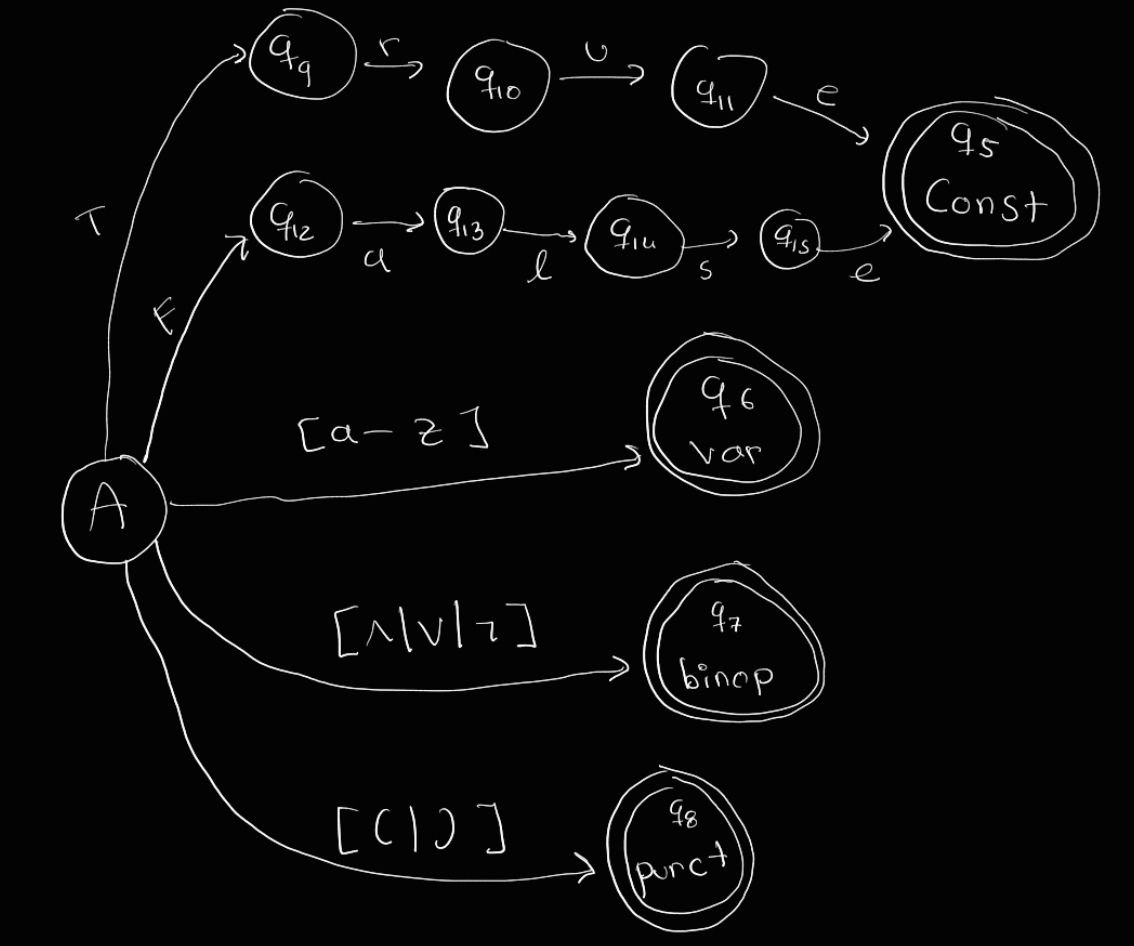
\includegraphics[width=0.8\textwidth]{images/ejercicio10-2.jpg}
    \caption{AFD para lexer expresiones booleanas}
    \label{fig:my_label}
\end{figure}


\textbf{Minimización del AFD}

Para minimizar el AFD, primero separamos los estados en dos grupos: los estados de aceptación y los que no lo son.

\begin{itemize}
    \item Grupo 1 (aceptación): $\{\{q_5, q_6, q_7, q_8\}\}$
    \item Grupo 2 (no aceptación): $\{A, \{q_9\}, \{q_{10}\}, \{q_{11}\}, \{q_{12}\}, \{q_{13}\}, \{q_{14}\}, \{q_{15}\}\}$
\end{itemize}

Como en el grupo 1 todos los estados son de aceptación, y no tienen transiciones es un grupo consistente. Ahora veamos como se comportarían los estados del Grupo 2 con las entradas posibles: 

\begin{table}[h!]
\centering
\begin{tabular}{|c|c|c|c|c|c|c|c|c|c|c|c|c|}
\hline
Estado &T & r & u & e & F & a & l &s &[a-z]-[r,u,e,a,l,s] &$\land/\lor/\lnot$ & (, )\\ \hline
\hline
$A$ & $\{q_9\}$ & $\{q_6\}$ & $\{q_6\}$ & $\{q_{6}\}$ & $\{q_{12}\}$ & $\{q_6\}$ & $\{q_6\}$ & $\{q_6\}$ & $\{q_6\}$ & $\{q_7\}$& $\{q_8\}$\\ \hline
$\{q_9\}$ & $\emptyset$ & $\{q_{10}\}$ & $\emptyset$ & $\emptyset$ & $\emptyset$  & $\emptyset$ & $\emptyset$ & $\emptyset$ & $\emptyset$ & $\emptyset$ & $\emptyset$\\ \hline
$\{q_{10}\}$ & $\emptyset$ &  $\emptyset$&  $\{q_{11}\}$& $\emptyset$ & $\emptyset$  & $\emptyset$ & $\emptyset$ & $\emptyset$ & $\emptyset$ & $\emptyset$ & $\emptyset$\\ \hline
$\{q_{11}\}$ & $\emptyset$ &  $\emptyset$& $\emptyset$ &  $\{q_{5}\}$& $\emptyset$  & $\emptyset$ & $\emptyset$ & $\emptyset$ & $\emptyset$ & $\emptyset$ & $\emptyset$\\ \hline
$\{q_{12}\}$ & $\emptyset$ & $\emptyset$ & $\emptyset$ & $\emptyset$  & $\emptyset$  & $\{q_{13}\}$ & $\emptyset$ & $\emptyset$& $\emptyset$ & $\emptyset$ & $\emptyset$\\ \hline
$\{q_{13}\}$ & $\emptyset$ &  $\emptyset$& $\emptyset$ & $\emptyset$ & $\emptyset$  & $\emptyset$ & $\{q_{14}\}$ & $\emptyset$ & $\emptyset$ & $\emptyset$ & $\emptyset$\\ \hline
$\{q_{14}\}$ & $\emptyset$ &  $\emptyset$& $\emptyset$ & $\emptyset$ & $\emptyset$  & $\emptyset$ & $\emptyset$ & $\{q_{15}\}$ & $\emptyset$ & $\emptyset$ & $\emptyset$\\ \hline
$\{q_{15}\}$ & $\emptyset$ &  $\emptyset$& $\emptyset$ & $\{q_{5}\}$ & $\emptyset$  & $\emptyset$ & $\emptyset$ & $\emptyset$ & $\emptyset$ & $\emptyset$ & $\emptyset$\\ \hline
\end{tabular}
\end{table}

Ahora si podemos los grupos de estados que se comportan igual:

\begin{table}[h!]
\centering
\begin{tabular}{|c|c|c|c|c|c|c|c|c|c|c|c|c|}
\hline
Estado &T & r & u & e & F & a & l &s &[a-z]-[r,u,e,a,l,s] &$\land/\lor/\lnot$ & (, )\\ \hline
\hline
$A$ & $ G_2$ & $ G_1$ & $G_1$ & $G_1$ & $G_2$ & $G_1$ & $G_1$ & $G_1$ & $G_1$ & $G_1$& $G_1$\\ \hline
$\{q_9\}$ & $\emptyset$ & $G_2$ & $\emptyset$ & $\emptyset$ & $\emptyset$  & $\emptyset$ & $\emptyset$ & $\emptyset$ & $\emptyset$ & $\emptyset$ & $\emptyset$\\ \hline
$\{q_{10}\}$ & $\emptyset$ &  $\emptyset$&  $G_2$& $\emptyset$ & $\emptyset$  & $\emptyset$ & $\emptyset$ & $\emptyset$ & $\emptyset$ & $\emptyset$ & $\emptyset$\\ \hline
$\{q_{11}\}$ & $\emptyset$ &  $\emptyset$& $\emptyset$ &  $G_1$& $\emptyset$  & $\emptyset$ & $\emptyset$ & $\emptyset$ & $\emptyset$ & $\emptyset$ & $\emptyset$\\ \hline
$\{q_{12}\}$ & $\emptyset$ & $\emptyset$ & $\emptyset$ & $\emptyset$  & $\emptyset$  & $G_2$ & $\emptyset$ & $\emptyset$& $\emptyset$ & $\emptyset$ & $\emptyset$\\ \hline
$\{q_{13}\}$ & $\emptyset$ &  $\emptyset$& $\emptyset$ & $\emptyset$ & $\emptyset$  & $\emptyset$ & $G_2$ & $\emptyset$ & $\emptyset$ & $\emptyset$ & $\emptyset$\\ \hline
$\{q_{14}\}$ & $\emptyset$ &  $\emptyset$& $\emptyset$ & $\emptyset$ & $\emptyset$  & $\emptyset$ & $\emptyset$ & $G_2$ & $\emptyset$ & $\emptyset$ & $\emptyset$\\ \hline
$\{q_{15}\}$ & $\emptyset$ &  $\emptyset$& $\emptyset$ & $G_1$ & $\emptyset$  & $\emptyset$ & $\emptyset$ & $\emptyset$ & $\emptyset$ & $\emptyset$ & $\emptyset$\\ \hline
\end{tabular}
\end{table}


Con la tabla anterior podemos agrupar los estados en los siguientes grupos:
\begin{itemize}
    \item $G_1 = \{\{q_6\}, \{q_7\}, \{q_8\}, \{q_5\}\}$
    \item $G_2 = \{A\}$
    \item $G_3 = \{q_9\}$
    \item $G_4 = \{q_{10}\}$
    \item $G_5 = \{q_{11},q_{15}\}$
    \item $G_6 = \{q_{12}\}$
    \item $G_7 = \{q_{13}\}$
    \item $G_8 = \{q_{14}\}$
\end{itemize}

Veamos como se comportarían los estados del Grupo $G_5$ con las entradas posibles:

\begin{table}[h!]
\centering
\begin{tabular}{|c|c|c|c|c|c|c|c|c|c|c|c|c|}
\hline
Estado &T & r & u & e & F & a & l &s &[a-z]-[r,u,e,a,l,s] &$\land/\lor/\lnot$ & (, )\\ \hline
\hline
$\{q_{11}\}$ & &  $\emptyset$& $\emptyset$ &  $G_1$& $\emptyset$  & $\emptyset$ & $\emptyset$ & $\emptyset$ & $\emptyset$ & $\emptyset$ & $\emptyset$\\ \hline
$\{q_{15}\}$ & &  $\emptyset$& $\emptyset$ & $G_1$ & $\emptyset$  & $\emptyset$ & $\emptyset$ & $\emptyset$ & $\emptyset$ & $\emptyset$ & $\emptyset$\\ \hline
\end{tabular}
\end{table}

Como son consistentes, y todos los otros grupos son unitarios, ya tenemos la tabla de transiciones del AFD mínimo:

\begin{table}[h!]
\centering
\begin{tabular}{|c|c|c|c|c|c|c|c|c|c|c|c|c|}
\hline
Estado &T & r & u & e & F & a & l &s &[a-z]-[r,u,e,a,l,s] &$\land/\lor/\lnot$ & (, )\\ \hline
\hline
$G_2$ & $ G_3$ & $ G_1$ & $G_1$ & $G_1$ & $G_6$ & $G_1$ & $G_1$ & $G_1$ & $G_1$ & $G_1$ & $G_1$\\ \hline
$G_1$ & $\emptyset$ & $\emptyset$ & $\emptyset$ & $\emptyset$ & $\emptyset$ & $\emptyset$ & $\emptyset$ & $\emptyset $ & $\emptyset$ & $\emptyset$ & $\emptyset$\\ \hline
$G_3$ & $\emptyset$ & $G_4$ & $\emptyset$ & $\emptyset$ & $\emptyset$  & $\emptyset$ & $\emptyset$ & $\emptyset$ & $\emptyset$ & $\emptyset$ & $\emptyset$\\ \hline
$G_4$ & $\emptyset$ &  $\emptyset$&  $G_5$& $\emptyset$ & $\emptyset$  & $\emptyset$ & $\emptyset$ & $\emptyset$ & $\emptyset$ & $\emptyset$ & $\emptyset$\\ \hline
$G_5$ & $\emptyset$ &  $\emptyset$& $\emptyset$ &  $G_1$& $\emptyset$  & $\emptyset$ & $\emptyset$ & $\emptyset$ & $\emptyset$ & $\emptyset$ & $\emptyset$\\ \hline
$G_6$ & $\emptyset$ & $\emptyset$ & $\emptyset$ & $\emptyset$  & $\emptyset$  & $G_7$ & $\emptyset$ & $\emptyset$& $\emptyset$ & $\emptyset$ & $\emptyset$\\ \hline
$G_7$ & $\emptyset$ &  $\emptyset$& $\emptyset$ & $\emptyset$ & $\emptyset$  & $\emptyset$ & $G_8$ & $\emptyset$ & $\emptyset$ & $\emptyset$ & $\emptyset$\\ \hline
$G_8$ & $\emptyset$ &  $\emptyset$& $\emptyset$ & $\emptyset$ & $\emptyset$  & $\emptyset$ & $\emptyset$ & $G_5$ & $\emptyset$ & $\emptyset$ & $\emptyset$\\ \hline
\end{tabular}
\caption{Tabla de transiciones del AFD mínimo}
\end{table}





Como queremos distinguir cada uno de los estados de aceptación, vamos a renombrar los grupos de la siguiente manera:


Con la tabla anterior podemos agrupar los estados en los siguientes grupos:
\begin{itemize}
    \item $G_{const}$ =  $\{q_5\}$
    \item $G_{var}$ =  $\{q_6\}$
    \item $G_{binop}$ =  $\{q_7\}$
    \item $G_{punct}$ =  $\{q_8\}$
    \item $G_2 = \{A\}$
    \item $G_3 = \{q_9\}$
    \item $G_4 = \{q_{10}\}$
    \item $G_5 = \{q_{11},q_{15}\}$
    \item $G_6 = \{q_{12}\}$
    \item $G_7 = \{q_{13}\}$
    \item $G_8 = \{q_{14}\}$
\end{itemize}

Veamos la tabla de transiciones final del AFD mínimo:

\begin{table}[h!]
    \centering
    \begin{tabular}{|c|c|c|c|c|c|c|c|c|c|c|c|c|}
    \hline
    Estado &T & r & u & e & F & a & l &s &[a-z]-[r,u,e,a,l,s] &$\land/\lor/\lnot$ & (, )\\ \hline
    \hline
    $G_2$ & $ G_3$ & $ G_{var}$ & $G_{var}$ & $G_{var}$ & $G_6$ & $G_{var}$ & $G_{var}$ & $G_{var}$ & $G_{var}$ & $G_{binop}$ & $G_{punct}$\\ \hline
    $G_{const}$ & $\emptyset$ & $\emptyset$ & $\emptyset$ & $\emptyset$ & $\emptyset$ & $\emptyset$ & $\emptyset$ & $\emptyset $ & $\emptyset$ & $\emptyset$ & $\emptyset$\\ \hline
    $G_{var}$ & $\emptyset$ & $\emptyset$ & $\emptyset$ & $\emptyset$ & $\emptyset$ & $\emptyset$ & $\emptyset$ & $\emptyset $ & $\emptyset$ & $\emptyset$ & $\emptyset$\\ \hline
    $G_{binop}$ & $\emptyset$ & $\emptyset$ & $\emptyset$ & $\emptyset$ & $\emptyset$ & $\emptyset$ & $\emptyset$ & $\emptyset $ & $\emptyset$ & $\emptyset$ & $\emptyset$\\ \hline
    $G_{punct}$ & $\emptyset$ & $\emptyset$ & $\emptyset$ & $\emptyset$ & $\emptyset$ & $\emptyset$ & $\emptyset$ & $\emptyset $ & $\emptyset$ & $\emptyset$ & $\emptyset$\\ \hline
    $G_3$ & $\emptyset$ &  $G_4$& $\emptyset$ & $\emptyset$ & $\emptyset$  & $\emptyset$ & $\emptyset$ & $\emptyset$ & $\emptyset$ & $\emptyset$ & $\emptyset$\\ \hline
    $G_4$ & $\emptyset$ &  $\emptyset$&  $G_5$& $\emptyset$ & $\emptyset$  & $\emptyset$ & $\emptyset$ & $\emptyset$ & $\emptyset$ & $\emptyset$ & $\emptyset$\\ \hline
    $G_5$ & $\emptyset$ &  $\emptyset$& $\emptyset$ &  $G_{const}$& $\emptyset$  & $\emptyset$ & $\emptyset$ & $\emptyset$ & $\emptyset$ & $\emptyset$ & $\emptyset$\\ \hline
    $G_6$ & $\emptyset$ & $\emptyset$ & $\emptyset$ & $\emptyset$  & $\emptyset$  & $G_7$ & $\emptyset$ & $\emptyset$& $\emptyset$ & $\emptyset$ & $\emptyset$\\ \hline
    $G_7$ & $\emptyset$ &  $\emptyset$& $\emptyset$ & $\emptyset$ & $\emptyset$  & $\emptyset$ & $G_8$ & $\emptyset$ & $\emptyset$ & $\emptyset$ & $\emptyset$\\ \hline
    $G_8$ & $\emptyset$ &  $\emptyset$& $\emptyset$ & $\emptyset$ & $\emptyset$  & $\emptyset$ & $\emptyset$ & $G_5$ & $\emptyset$ & $\emptyset$ & $\emptyset$\\ \hline
    \end{tabular}
    \caption{Tabla de transiciones del AFD mínimo renombrado}
\end{table}


Obtenemos entonces el siguiente autómata:

\begin{figure}[h!]
    \centering
    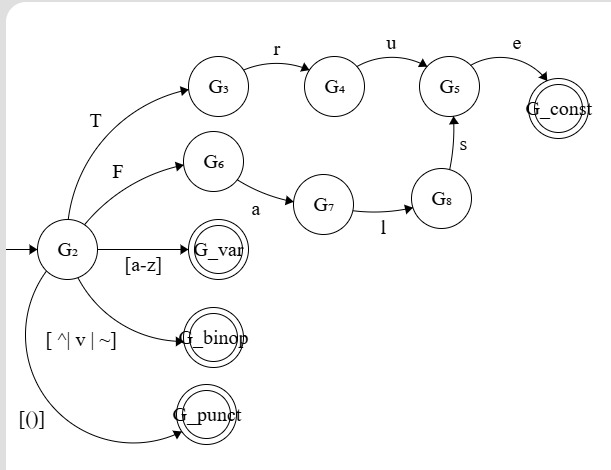
\includegraphics[width=0.8\textwidth]{images/ej10-3.jpeg}
    \caption{AFD mínimo para lexer expresiones booleanas}
    \label{fig:my_label}
\end{figure}


Vamos a hacer la prueba del AFD mínimo con las expresiones dadas. Seguiremos la regla de la coincidencia más larga.

\begin{enumerate}
    \item \textbf{Inicio:} Se empieza en el estado inicial del autómata y en el primer carácter de la cadena pendiente de procesar.

    \item \textbf{Consumo y Registro:} Se lee un carácter a la vez y se avanza al siguiente estado según las transiciones del autómata.
    \begin{itemize}
        \item \textbf{Importante:} Cada vez que se pasa por un estado de aceptación, se guardan en una variable dos cosas: el tipo de token de ese estado (ej: CONST, VAR) y la posición actual en la cadena.
    \end{itemize}

    \item \textbf{Avance hasta atorarse:} Se siguen consumiendo caracteres hasta encontrar una situación donde, para el siguiente carácter de la entrada, no existe una transición válida desde el estado actual. A esto se le llama atorarse o llegar a un estado de error/sumidero.

    \item \textbf{Retroceso y Corte:} Cuando se atoran, el proceso se detiene. En ese momento, se consulta el último estado de aceptación que fue guardado:
    \begin{itemize}
        \item El token encontrado es la subcadena que va desde el inicio del análisis hasta la posición guardada.
        \item El tipo de token es el que se guardó en ese momento.
    \end{itemize}

    \item \textbf{Emisión y Repetición:} Se "emite" el token encontrado. Luego, el puntero de la cadena de entrada se mueve al carácter que sigue al final de ese token y se vuelve a empezar el proceso desde el paso 1.
\end{enumerate}



\begin{enumerate}
    \item[(a)] $p \land q$
    
    \begin{itemize}
        \item Comenzamos leyendo 'p', nos movemos al estado $G_{var}$ (aceptación VAR), guardamos token VAR y posición 1.
        \item Leemos espacio ' ', no hay transición desde $G_{var}$, nos atoramos.
        \item Retrocedemos a posición 1, emitimos token VAR con valor 'p'.
        \item Avanzamos al siguiente carácter (espacio), no hay transición desde estado inicial, nos atoramos.
        \item No hay token guardado para el espacio.
        \item Avanzamos al siguiente carácter 'a', nos movemos al estado $G_{binop}$ (aceptación BINOP), guardamos token BINOP y posición 3.
        \item Leemos espacio ' ', no hay transición desde $G_{binop}$, nos atoramos.
        \item Retrocedemos a posición 3, emitimos token BINOP con valor '$\land$'.
        \item Avanzamos al siguiente carácter (espacio), no hay transición desde estado inicial, nos atoramos.
        \item No hay token guardado para el espacio.
        \item Avanzamos al siguiente carácter 'q', nos movemos al estado $G_{var}$ (aceptación VAR), guardamos token VAR y posición 5.
        \item Llegamos al final de la cadena, emitimos token VAR con valor 'q'.
    \item \textbf{Tokens emitidos:}
        \begin{itemize}
            \item VAR: 'p'
            \item BINOP: '$\land$'
            \item VAR: 'q'
        \end{itemize}
    \end{itemize}


    \item[(b)] $\textbf{True} \land \lnot(p \lor q)$
    \item[(c)] $\lnot(x \land y) \lor (p \land q)$
\end{enumerate}